\documentclass[conference]{IEEEtran}
\IEEEoverridecommandlockouts
% The preceding line is only needed to identify funding in the first footnote. If that is unneeded, please comment it out.
\usepackage{cite}
\usepackage[portuges,brazil,english]{babel}
\usepackage[utf8]{inputenc}
\usepackage{amsmath,amssymb,amsfonts}
%\usepackage{algorithmic}
\usepackage{graphicx}
\usepackage{textcomp}
\def\BibTeX{{\rm B\kern-.05em{\sc i\kern-.025em b}\kern-.08em
    T\kern-.1667em\lower.7ex\hbox{E}\kern-.125emX}}
\begin{document}

\title{Predição do Ano de Músicas a Partir de Timbres}

\author{\IEEEauthorblockN{André Almeida}
\IEEEauthorblockA{
RA: 164047 \\
\texttt{fda.andre@gmail.com}}
\and
\IEEEauthorblockN{Igor Torrente}
\IEEEauthorblockA{
RA: 169820 \\
\texttt{igortorrente@hotmail.com}}}

\maketitle

\section{Introdução}

Nesse trabalho, estudamos técnicas de aprendizado de máquina para obter um modelo linear que prediz o ano de uma música com base em diversos métricas de timbre, armazenadas em um banco de dados populado com diversas amostras de músicas comerciais entre 1922-2010. Foram estudados diversos algoritmos lineares e subconjuntos de treino para comparação de resultados.\\
Utilizamos a biblioteca \textit{sklearn}\cite{b1} do \textit{Python}, que já contem implementações de diversos algoritmos de aprendizado de máquina, além de funções de métricas e preprocessamento. Foi utilizado para importar os dados do arquivo \texttt{csv} a biblioteca \textit{Pandas}. O \textit{Jupyter} foi escolhido como ambiente de desenvolvimento.\\
Os recurso computacional disponível foi um computador com um processador Intel Core i7-3537U (2.00GHz × 4) e com 7,7 GiB disponíveis de memória RAM.

%\section{Atividades}
%
%The state-of-the-art research (about prior work for solving the same problem).

\section{Dados}
A base de dados contém no total 499.973 amostras, com o ano da música e 90 atributos, sendo destes: 12 médias de timbre e 78 covariâncias de timbre. O banco de dados foi obtido a partir do LabROSA\cite{b2}, da Columbia University. Os dados foram dividos como 93,2\% para treino e 7,8\% para teste.\\
Adicionamos, para facilitar a manipulação dos dados, cabeçalhos às colunas do banco. A primeira coluna de ano foi nomeada \texttt{year}, as 12 colunas de médias de timbres \texttt{ta01}...\texttt{ta12} e as 78 colunas de covariância \texttt{tc01}...\texttt{tc78}. \\
Separamos os dados de treino como 80\% de treino e 20\% para validação. Embaralhamos os dados para evitar qualquer ordenação no banco de dados original, que pudesse deixar algum viés. Os dados do treino foram usados apenas uma vez, após os testes com a validação.  Os \textit{scores} e percentagem dos acertos descritos no artigo são referentes ao conjunto de testes.\\
O ano das músicas é o \textit{y} (ou \textit{f(x)}) e os 90 parâmetros são o \textit{x}. Conforme orientado em \cite{b3}, no capítulo de \textit{Gradient Descent}, aplicamos uma normalização (\texttt{StandardScaler}) que normaliza os dados para não haver maior influência dos que variam mais, assim melhorando a convergência da função.\\
Existe um pico de músicas na década de 2000, levando essa década a ter uma variabilidade maior nos dados. Além disso, acredita-se que devido o avanço das técnicas de gravação e produção sonora durante o tempo, isso permitiu músicas com variedades de timbres mais complexas.

\begin{center}
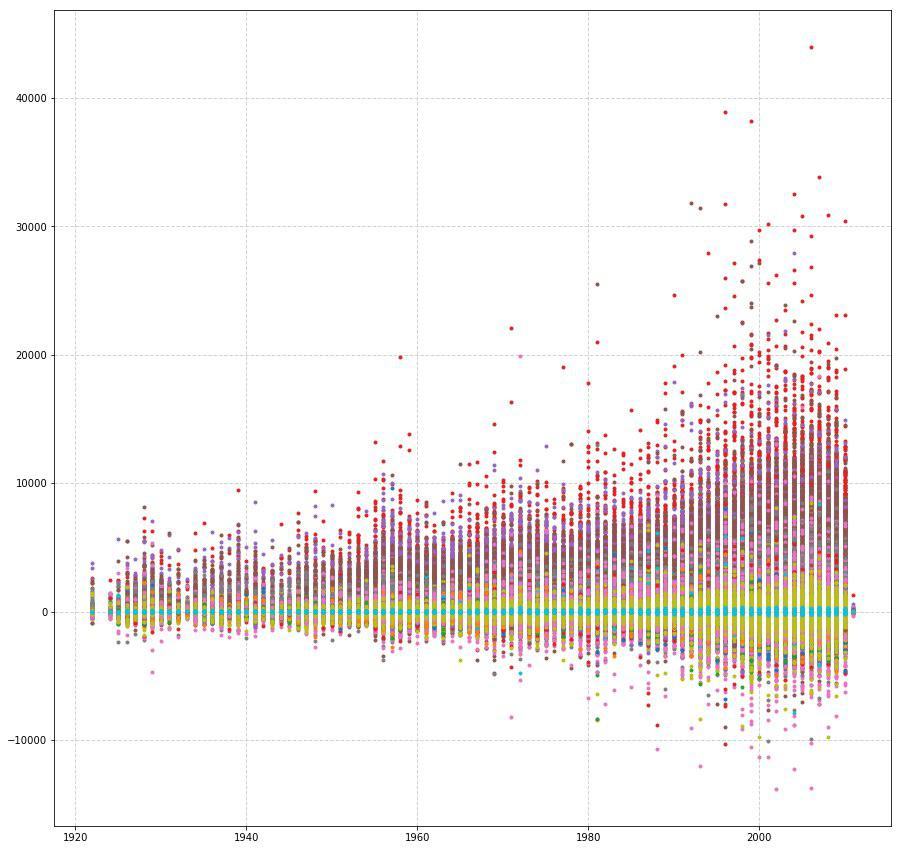
\includegraphics[scale=0.25]{plot0}
\\
\textbf{Figura 1: Valores da 90 features (cada uma representada por uma cor) x por ano}
\end{center}


\section{Soluções propostas}
Nessa sessão e nas próximas, \textit{score} é a métrica de acerto do dado definida como o coeficiente de determinação R². O coeficiente R² é calculado como $(1 - u/v)$, onde $u$ é a soma residual dos quadrados $(y_{real} - y_{predito})^2$ e $v$ é a soma total dos quadrados $(y_{real} - media(y_{real})^2$, para todos os $y$. O melhor valor possível é 1, e pode ser arbitrariamente negativo.\cite{b4}

\subsection{Regressão linear com descida estocástica de gradiente}
Utilizando o módulo \texttt{linear\_model.SGDRegressor}, aplicamos uma decida de gradiente na função de custo de uma regressão linear e obtivemos uma função. Utilizamos uma taxa de aprendizado de  $10^{-4}$ e o número máximo de iterações igual a 100, e obtivemos o score mais alto no conjunto de validação: 0.2331. Os outros parâmetros não foram alterados pois não contribuíam com alterações nos resultados. Foram testados outros valores, mas que não convergiram tão bem:
\begin{center}

\begin{tabular}{ l c r }
  \texttt{eta0} & \texttt{max\_iter} & score \\
  $10^{-6}$ & 50 & -15775.02 \\
  $10^{-3}$ & 200 & 0.2293 \\
  $10^{-5}$ & 150 & 0.2297 \\
\end{tabular}

\end{center}

No conjunto de testes, o score final foi de \textbf{0.2293} com \textbf{5.18\%} de acerto.\\

\begin{center}
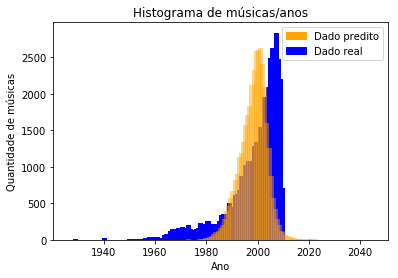
\includegraphics[scale=0.6]{plot1}
\textbf{Figura 2: histograma da primeira solução}
\\
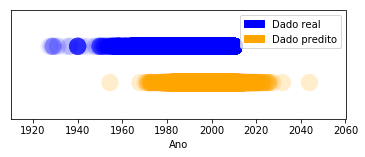
\includegraphics[scale=0.6]{plot2}
\textbf{Figura 3: distribuição dos anos nos conjuntos}

\end{center}


\subsection{Regressão linear com Lasso}
Lasso \cite{b5} é um método linear que usa o erro L1 (erro absoluto) como regularizador. Utilizamos o \texttt{linear\_model.Lasso} em nosso código, mudando apenas o parâmetro \texttt{alpha}, deixando com o valor \texttt{0.0001}. Lasso é considerado como um modelo mais poderoso, por regularizar os dados previamente antes de aplicar a regressão linear. Obtivemos como score no teste \textbf{0.2292} e acerto \textbf{5.17\%}.

\begin{center}
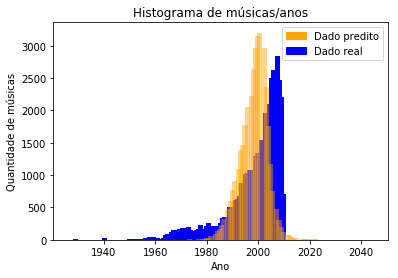
\includegraphics[scale=0.6]{plot3}
\textbf{Figura 4: histograma da segunda solução}
\\
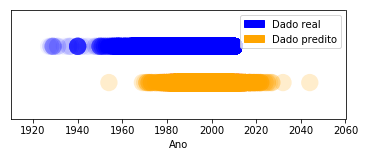
\includegraphics[scale=0.6]{plot4}
\textbf{Figura 5: distribuição dos anos nos conjuntos}

\end{center}

\subsection{Regressão linear com Equação Normal}
Para testarmos a regressão linear com a decida de equação normal,  usamos a função \texttt{linear\_model.LinearRegression}, que já implementa por padrão a equação normal para minimizar o erro. Mantemos o parâmetro \texttt{Normalize} desativado, já que não ele promoveu nenhuma alteração no resultado. Usamos os conjuntos de dados sem a regularização, obtendo um score ligeiramente maior (0.001\%). Os resultados finais foram: score  \textbf{0.2297} e acerto de \textbf{5.24\%}.

\begin{center}
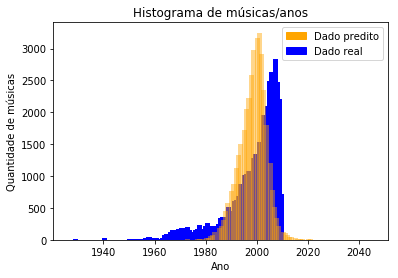
\includegraphics[scale=0.6]{plot5}
\textbf{Figura 6: histograma da segunda solução}
\\
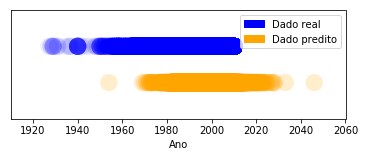
\includegraphics[scale=0.6]{plot6}
\textbf{Figura 7: distribuição dos anos nos conjuntos}
\end{center}

Na figura 8 podemos ver a diferença entre o valor real e o valor predito no nosso modelo. Um modelo com \textit{overfitting} apresentaria uma reta perfeita crescente.

\begin{center}
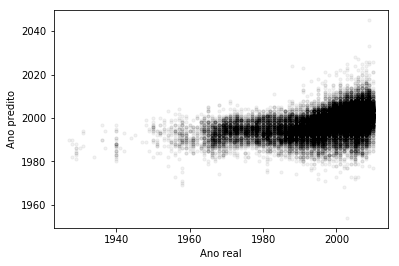
\includegraphics[scale=0.6]{plot7}
\textbf{Figura 8: anos preditos x anos reais}
\end{center}

\section{Descida de gradiente}
Tanto os modelos automáticos (\texttt{linear\_model.Lasso} e \texttt{linear\_model.LinearRegression}) tanto o modelo manual (\texttt{linear\_model.SGDRegressor}) tiveram resultados muito próximos da descida de gradiente/equação normal, já que observamos scores muito próximos.

\begin{center}
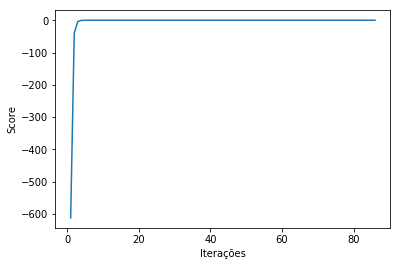
\includegraphics[scale=0.6]{plot8}
\textbf{Figura 9: Score x Número de iterações \\ (\texttt{SGDRegressor)}}
\end{center}

\section{Resultados}
  Nos gráficos [2-4-6] temos um histograma comparativo da predição do nosso modelos (laranja) e os dados reais (azul), que mostra que nossos modelos não predizem a quantidade correta de músicas nos seu respectivos anos. Nosso modelo se assemelha a uma gaussiana um pouco deslocada para a esquerda.\\
  Nos gráficos [3-5-7] temos a concentração das predições dos modelos (laranja) e dos dados reais (azul) baseado na tonalidade da cor, demonstrando uma relativamente alta predição do nosso modelo depois do ano de 2011 e uma baixa predição nos anos entre 1922 a 1965. O modelo parece "descolar" os anos cerca de três décadas à frente.
\subsection{Descida de gradiente estocástica}
  Como visto anteriormente na sessão de resultados, conseguimos um score e uma precisão baixa tanto nas validações quanto no teste e a proporção de treino e validação não influenciou a precisão dos modelos, indicando que ele é muito simples e não se adequa corretamente aos nossos dados, observa-se um claro underfiting.

\subsection{Lasso e Normal}
  A conclusão dada a descida de gradiente estocástica se aplica ao método de Lasso e a Normal com resultados de score e precisão também muito próximos, podendo ser observado pela similaridade os gráficos de todos os modelos obtidos com as três técnicas.

\subsection{Análise dos erros}
Analisamos os erros no \texttt{LinearRegression}. Das 34384 predições erradas, 13922 (40,4\%) erraram para um ano maior do que o real, e 20462 (58,7\%) erraram para um ano menor. Dos erros para cima, a média foi de 8.89 anos, e para baixo, de 6.05 anos. Os erros por décadas podem ser vistos na tabela abaixo:

\begin{center}

\begin{tabular}{ l | c}
\textbf{Década} & \textbf{Erro} \\
1920 & 12 \\
1930 & 704 \\
1940 & 19949 \\
1950 & 8055 \\
1960 & 2876 \\
1970 & 1694 \\
1980 & 838 \\
1990 & 207 \\
2000 & 39 \\
2010 & 10
\end{tabular}

\end{center}


Uma possível explicação seria o fato do grande aglomerado de músicas a partir do século XXI no banco criarem um viés para "cima" e a falta de dados antigos tornam eles menos precisos.

\section{Conclusão}
Nenhum modelo linear foi capaz de criar funções que predizem corretamente o ano a partir da base de dados usadas, mas o adequado entre eles foi a Regressão linear com Equação Normal (\texttt{linear\_model.LinearRegression}), com um score  \textbf{0.2297} e acerto de \textbf{5.24\%}.

\section{Estudos futuros}
Precisamos de mais estudo sobre os dados para descobrimos mais o comportamento e correlação entre eles, uso de técnicas de pré-processamento para removermos dados pouco relevantes e inter-relacionados entre si. Também é necessário mais hardware e modelos mais complexos (árvore de decisão, polinomial) que se ajustam melhor ao problema. Uma possível alternativa seria alterar 


%\section{Experiments and Discussion}
%
%The experiments carried out and the obtained
%results.
%
%\section{Conclusions and Future Work}
%
%The main conclusions of the work as well as some future directions for other people interested in continuing this work. 

\begin{thebibliography}{00}

\bibitem{b1} Scikit-learn: Machine Learning in Python, acessado em 31 de Agosto de 2017, em \texttt{http://scikit-learn.org/stable/index.html}

\bibitem{b2} Million Song Dataset, em: http://labrosa.ee.columbia.edu/millionsong/

\bibitem{b3}  Geron, A. (2017). \textit{Hands-on machine learning with Scikit-Learn and TensorFlow: concepts, tools, and techniques to build intelligent systems.}

\bibitem{b4} Scikit-learn: sklearn.linear\_model.LinearRegression, acessado em 31 de Agosto de 2017, em http://scikit-learn.org/stable/modules/generated/sklearn.linear\_model.LinearRegression.html

\bibitem{b5}  Scikit-learn: sklearn.linear\_model.Lasso, acessado em 31 de Agosto de 2017, em http://scikit-learn.org/stable/modules/generated/sklearn.linear\_model.Lasso.html

\end{thebibliography}

\end{document}
